\documentclass[10pt,a4paper]{article}
\usepackage[margin=0.75in,top=0.7in,bottom=0.7in]{geometry}
\usepackage[T1]{fontenc}
\usepackage{lmodern}
\usepackage{amsmath}
\usepackage{graphicx}
\usepackage{booktabs}
\usepackage{array}
\usepackage{caption}
\usepackage{hyperref}
\usepackage{xcolor}
\usepackage{titlesec}
\usepackage{enumitem}
\usepackage{float}

\captionsetup{font=small,labelfont=bf,skip=2pt}
\titlespacing*{\section}{0pt}{7pt}{3pt}
\titleformat{\section}{\large\bfseries}{\thesection}{0.6em}{}
\setlength{\parskip}{3pt}\setlength{\parindent}{0pt}
\setlist{nosep,leftmargin=1.2em}
\hypersetup{colorlinks=true,linkcolor=black,urlcolor=blue!50!black}
\graphicspath{{figures/}}

% ====== FILL IN BEFORE SUBMITTING ===========================================
\newcommand{\memberA}{Member 1 Name (Roll No.)}
\newcommand{\memberB}{Member 2 Name (Roll No.)}
\newcommand{\githuburl}{https://github.com/YOUR-USERNAME/hids-project}
\newcommand{\streamlithurl}{https://YOUR-APP.streamlit.app}
\newcommand{\hfspaceurl}{https://huggingface.co/spaces/YOUR-USERNAME/hids-demo}
\newcommand{\hfmodelurl}{https://huggingface.co/YOUR-USERNAME/hids-nsl-kdd-classifier}
% =============================================================================

% Screenshot helper: shows the image if the file exists, otherwise a placeholder box
\newcommand{\shot}[2]{\IfFileExists{figures/#1}{\includegraphics[width=\linewidth]{#1}}{%
  \fbox{\parbox[c][2.6cm][c]{0.9\linewidth}{\centering\small\textcolor{red}{Insert screenshot:\ #2\\(save as \detokenize{figures/#1})}}}}}

\begin{document}

\begin{center}
{\LARGE\bfseries Host-Based Intrusion Detection \& Automated Response System (HIDS)}\\[3pt]
CT-378 Machine Learning --- Semester Project Report\\[2pt]
\memberA\ \ $\cdot$\ \ \memberB\\[2pt]
{\small Code: \url{\githuburl}}
\end{center}

\begin{abstract}\noindent
We built a machine-learning intrusion detector that labels each host/connection record as \emph{Normal}, \emph{DoS},
\emph{Probe}, \emph{R2L} (remote-to-local, e.g.\ password guessing) or \emph{U2R} (user-to-root privilege escalation) and maps
the verdict to an automated response plan. Using 147{,}888 de-duplicated NSL-KDD records (41 features) we compared a majority-class
baseline with Logistic Regression, Random Forest and Histogram Gradient Boosting inside a leak-free scikit-learn pipeline with
5-fold GridSearchCV. The tuned Random Forest reached \textbf{99.5\% accuracy and 0.921 macro-F1} (ROC-AUC 0.999) on a held-out test set.
The rare U2R class is the weak point (F1 0.67). The model is deployed through Streamlit, a Hugging Face Space and a local Flask web app.
\end{abstract}

\section{Problem and motivation}
A host-based intrusion detection system (HIDS) watches activity on a machine and raises alarms when behaviour looks malicious.
Rule/signature tools miss new patterns and generate many false alarms, while analysts cannot react to every event. We therefore
frame detection as a \emph{multi-class classification} problem and add an \emph{automated response} layer: each predicted
class triggers a policy (e.g.\ DoS $\rightarrow$ block source; U2R $\rightarrow$ terminate session and isolate host; low-confidence
verdicts $\rightarrow$ analyst review). The intended user is a system administrator or SOC analyst. The success metric is
\textbf{macro-F1}, because 52\% of records are normal and the attack classes are very unbalanced; accuracy alone would hide
failures on rare attacks.

\section{Data collection}
We first tried to capture and label traffic from our own machine while running brute-force, privilege-escalation and reverse-shell
attacks, but could not obtain a reliable labelled data set in the available time. We therefore used the public
\textbf{NSL-KDD} benchmark \cite{tavallaee2009}, a cleaned version of KDD Cup 1999 that contains \emph{host-level} features
(\texttt{num\_failed\_logins}, \texttt{root\_shell}, \texttt{su\_attempted}, \texttt{num\_shells}, \dots) next to traffic statistics.
Two public files, \texttt{KDDTrain+} (125{,}973 rows) and \texttt{KDDTest+} (22{,}544 rows), were downloaded from a public GitHub mirror
(\texttt{github.com/defcom17/NSL\_KDD} \cite{mirror}) on 22 Nov 2026 with a download script, and pooled. The data is released by the Canadian
Institute for Cybersecurity for research use and contains no personal identifiers (no IPs or user names).
Pooling revealed 629 exact duplicates across the two files, which we removed to prevent train/test leakage, leaving
\textbf{147{,}888 rows $\times$ 41 features} (3 categorical, 38 numeric) with no missing values. The $\sim$40 attack names were mapped to five
classes: Normal (52.0\%), DoS (35.8\%), Probe (9.4\%), R2L (2.6\%), U2R (0.08\%, 119 rows).

\section{Exploratory data analysis}
Figure~\ref{fig:eda} summarises six analyses (class balance, protocol mix, outliers, error rates, host indicators, correlations).
(i) The data are strongly imbalanced, so we use class weights and macro-F1. (ii) \texttt{src\_bytes} is heavy-tailed with extreme outliers
in every class, motivating a log transform. (iii) DoS records have SYN-error rates near 1, a clear signature; R2L shows failed/guest logins;
U2R shows root-shell, \texttt{su} and file-creation activity. (iv) Many \texttt{*\_rate} features are highly correlated (13 pairs
with $|r|>0.9$), which suits tree models and regularised linear models. (v) One numeric column (\texttt{num\_outbound\_cmds}) is constant.
\begin{figure}[H]\centering
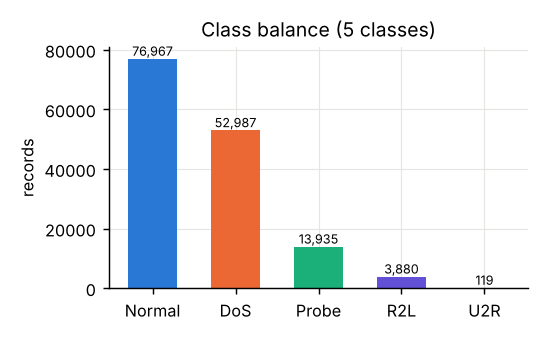
\includegraphics[width=0.32\linewidth]{eda_class_balance.png}\hfill
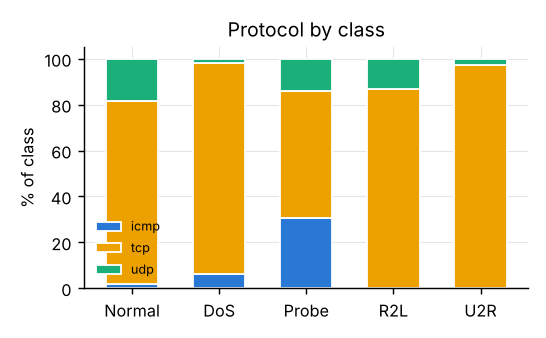
\includegraphics[width=0.32\linewidth]{eda_protocol.png}\hfill
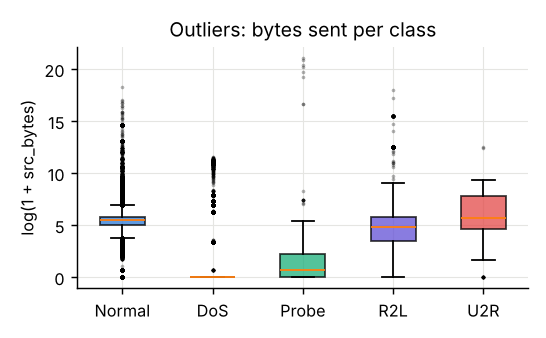
\includegraphics[width=0.32\linewidth]{eda_bytes_boxplot.png}\\[2pt]
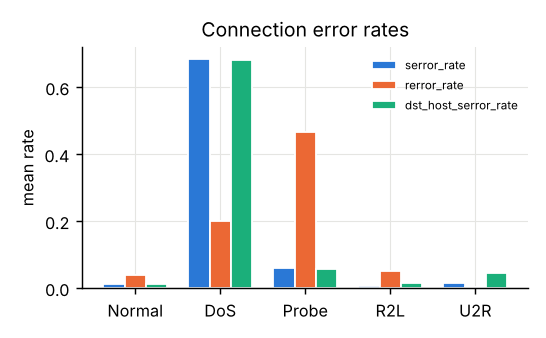
\includegraphics[width=0.32\linewidth]{eda_error_rates.png}\hfill
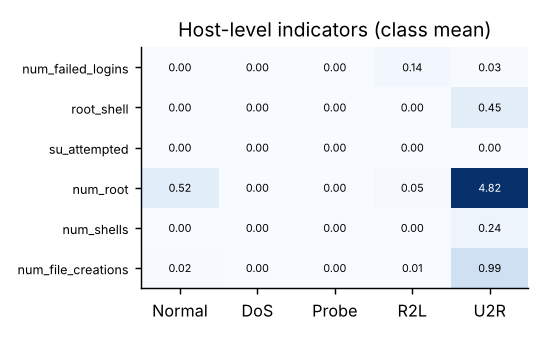
\includegraphics[width=0.32\linewidth]{eda_host_indicators.png}\hfill
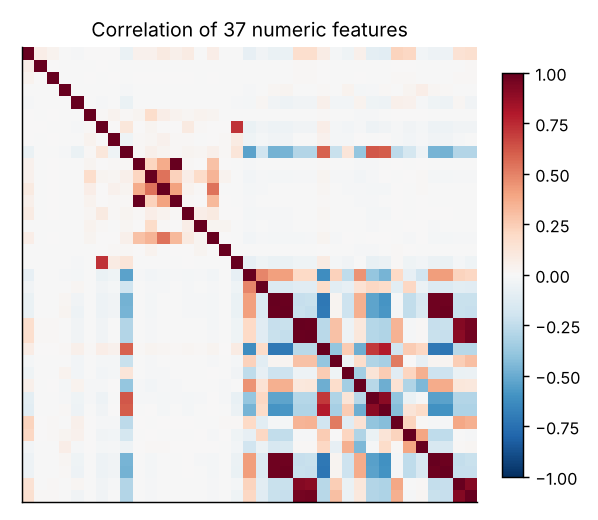
\includegraphics[width=0.30\linewidth]{eda_correlation.png}
\caption{EDA: class balance, protocol by class, outliers in $\log(\text{src\_bytes})$, error rates, host-level indicators, correlation.}
\label{fig:eda}
\end{figure}

\section{Methodology}
\textbf{Split.} Stratified 70/15/15 train/validation/test (103{,}521 / 22{,}183 / 22{,}184 rows), random seed 42.
\textbf{Pipeline} (one scikit-learn \texttt{Pipeline}, fitted on training data only): (1) feature engineering---$\log(1{+}\text{src\_bytes})$,
$\log(1{+}\text{dst\_bytes})$, log byte ratio, a privilege score (root shell + \texttt{su} + root/file/shell counts) and mean error rate;
(2) median/most-frequent imputation (a safeguard for blank inputs in the apps); (3) standard scaling of numerics and one-hot encoding of
\texttt{protocol\_type}, \texttt{service}, \texttt{flag}; (4) classifier.
\textbf{Models.} Baseline = majority class; then Logistic Regression, Random Forest \cite{breiman2001} and Histogram Gradient Boosting
\cite{friedman2001}, all with balanced class weights. \textbf{Tuning.} 5-fold stratified GridSearchCV on the training set,
scoring macro-F1 (Table~\ref{tab:cmp}); all code uses scikit-learn \cite{pedregosa2011}. The model was chosen on the validation set; the test set was used once, for the chosen model.

\section{Results}
\begin{table}[H]\centering\small
\caption{Model comparison (macro-F1 unless stated). The test set is not used here.}\label{tab:cmp}
\begin{tabular}{lllcccc}\toprule
Model & Best parameters & CV & Train & Val & Val acc.\\\midrule
Baseline (majority) & --- & --- & 0.137 & 0.137 & 0.520\\
Logistic Regression & $C=10$ & 0.743 & 0.748 & 0.742 & 0.951\\
Random Forest & depth=None, min\_leaf=3 & 0.929 & 0.970 & \textbf{0.949} & 0.994\\
Hist.\ Gradient Boosting & lr=0.15, leaves=15 & 0.915 & 0.961 & 0.922 & 0.992\\\bottomrule
\end{tabular}
\end{table}
\textbf{Under/over-fitting.} Logistic Regression underfits (train $\approx$ validation $\approx$ 0.74): the classes are not linearly separable.
Random Forest and boosting fit well; the 0.02--0.04 train--validation gap is small and CV agrees with validation, so overfitting is mild.
The Random Forest was selected.

\textbf{Test performance (held-out, used once).} Accuracy 0.9949, macro-F1 0.9205, weighted-F1 0.9949, ROC-AUC (one-vs-rest) 0.9986.
Table~\ref{tab:cls} gives per-class scores and Figure~\ref{fig:res} the confusion matrix and the most important features.
\begin{table}[H]\centering\small
\caption{Test-set results of the Random Forest per class.}\label{tab:cls}
\begin{tabular}{lcccc}\toprule
Class & Precision & Recall & F1 & Support\\\midrule
Normal & 0.998 & 0.993 & 0.995 & 11{,}545\\
DoS & 0.999 & 1.000 & 0.999 & 7{,}948\\
Probe & 0.987 & 0.999 & 0.993 & 2{,}091\\
R2L & 0.926 & 0.973 & 0.949 & 582\\
U2R & 0.667 & 0.667 & 0.667 & 18\\\bottomrule
\end{tabular}
\end{table}
\begin{figure}[H]\centering
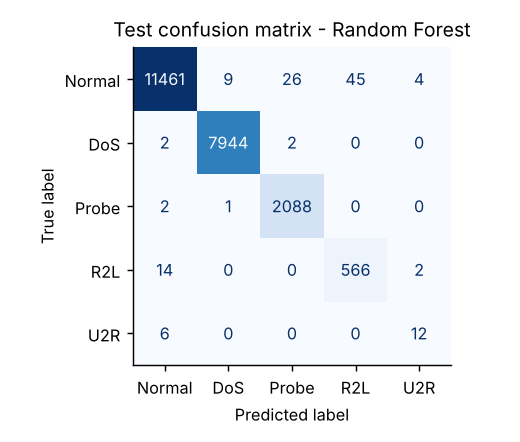
\includegraphics[width=0.32\linewidth]{confusion_matrix.png}\hfill
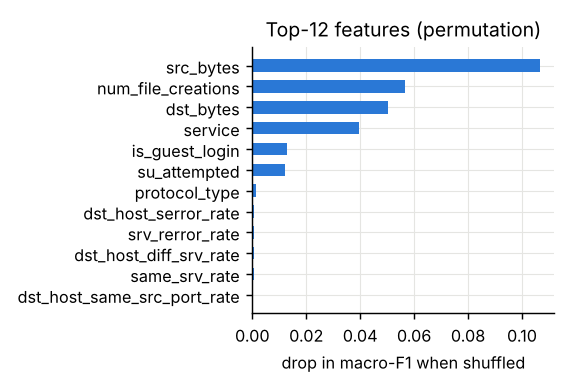
\includegraphics[width=0.32\linewidth]{feature_importance.png}\hfill
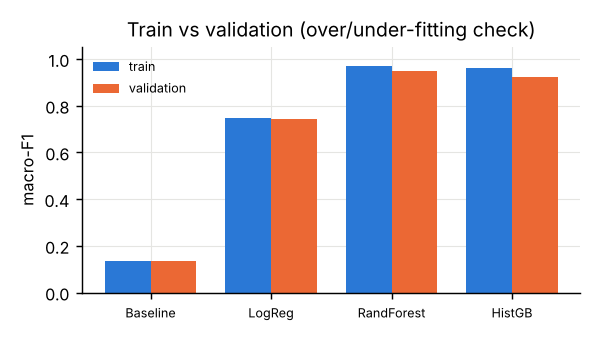
\includegraphics[width=0.32\linewidth]{model_comparison.png}
\caption{Left: test confusion matrix. Middle: top-12 features by permutation importance (validation data). Right: train vs.\ validation macro-F1.}
\label{fig:res}
\end{figure}
\textbf{Error analysis.} Only 113 of 22{,}184 test records are misclassified. The largest groups are Normal$\rightarrow$R2L (45) and
Normal$\rightarrow$Probe (26) (false alarms), then R2L$\rightarrow$Normal (14) and U2R$\rightarrow$Normal (6) (missed attacks).
U2R has just 18 test records, so its F1 is very unstable: one more mistake changes it noticeably. Most important features are
\texttt{src\_bytes}, \texttt{num\_file\_creations}, \texttt{dst\_bytes}, \texttt{service}, \texttt{is\_guest\_login} and \texttt{su\_attempted},
which agree with the EDA.

\section{Deployment}
The same pipeline (saved with \texttt{joblib}; versions pinned in \texttt{requirements.txt}) and the same response engine are used by three
front ends. Each takes the 12 most important features (the other 29 default to typical training values or to a chosen real example),
returns the predicted class with its probability, and shows the response plan. Responses are simulated: they are displayed and logged, not
executed on a firewall; verdicts below 60\% confidence become ``manual review''.
\begin{itemize}
\item \textbf{Streamlit:} form, probability chart, importance chart and CSV batch tab --- \url{\streamlithurl}
\item \textbf{Hugging Face:} model card and pipeline \url{\hfmodelurl}; live Gradio Space \url{\hfspaceurl}
\item \textbf{Local Flask app:} \texttt{POST /predict} with JSON validation (HTTP 422 with messages for bad types, unknown categories, negative or out-of-range values) and an HTML front end on \texttt{localhost:5000}.
\end{itemize}
\begin{figure}[H]\centering
\begin{minipage}{0.32\linewidth}\shot{shot_streamlit.png}{Streamlit app with a prediction}\end{minipage}\hfill
\begin{minipage}{0.32\linewidth}\shot{shot_hf.png}{Hugging Face Space}\end{minipage}\hfill
\begin{minipage}{0.32\linewidth}\shot{shot_flask.png}{Flask app on localhost}\end{minipage}
\caption{Screenshots of the three deployments.}
\end{figure}

\section{Limitations and future work}
\begin{itemize}
\item \textbf{Old, benchmark data.} NSL-KDD derives from 1998 traffic and mostly describes network connections with host-level fields; it is not live data from a modern host, and our own capture of host attacks was not completed. The apps are demonstrations, not a deployable security product.
\item \textbf{Optimistic evaluation.} Our random split of pooled data shares attack types between train and test. The official \texttt{KDDTest+} contains unseen attack variants and is known to be harder, so real-world performance would be lower.
\item \textbf{Rare classes.} U2R has about 120 records; its metrics have very high variance and 6 of 18 test cases were missed.
\item \textbf{Simulated response.} The policy is rule-based and does not act on a real system.
\end{itemize}
\textbf{Future work:} collect labelled logs/system-call traces from a lab VM, evaluate on unseen attack types, apply resampling (e.g.\ SMOTE) or cost-sensitive thresholds for U2R, add explanations (SHAP) and connect the response engine to a real firewall API.

\section*{Individual contributions}
\begin{center}\begin{tabular}{p{3.4cm}p{12.2cm}}\toprule
Member & Contribution\\\midrule
\memberA & Data download and cleaning, EDA, pipeline and model tuning, evaluation, report\\
\memberB & Response engine, Streamlit / Flask / Hugging Face deployments, testing, documentation\\\bottomrule
\end{tabular}\end{center}
{\small\textit{(Edit this table to match who actually did what --- every member must be able to explain all parts in the viva.)}}

\begin{thebibliography}{9}\small
\bibitem{tavallaee2009} M.~Tavallaee, E.~Bagheri, W.~Lu, A.~Ghorbani, ``A detailed analysis of the KDD CUP 99 data set,'' \textit{IEEE Symp.\ on Computational Intelligence for Security and Defense Applications (CISDA)}, 2009.
\bibitem{pedregosa2011} F.~Pedregosa et al., ``Scikit-learn: Machine learning in Python,'' \textit{J.\ Machine Learning Research}, 12:2825--2830, 2011.
\bibitem{breiman2001} L.~Breiman, ``Random forests,'' \textit{Machine Learning}, 45(1):5--32, 2001.
\bibitem{friedman2001} J.~H.~Friedman, ``Greedy function approximation: a gradient boosting machine,'' \textit{Annals of Statistics}, 29(5):1189--1232, 2001.
\bibitem{mirror} NSL-KDD files mirror: \url{https://github.com/defcom17/NSL_KDD} (accessed 22 Nov 2026).
\end{thebibliography}
\end{document}
